\part{Analysis}  \label{part:analysis}

\chapter{Methodology}

In this chapter, we will present the methodology used to analyze our solution. Our tests were focused on data retrieval, as we considered it to be the part that needed to be evaluated the most. This is mainly due to the fact that our solution will be considered viable only if it does not stress intensively the network. Because we are talking about Internet of Things and particularly Wireless Sensors Network, preserving the battery life of nodes is a must. This can be done by maximizing the CPU sleep time, or reducing the transmission or reception time. For those particular reasons, four criteria designed our tests:

\begin{itemize}
  \item CPU duty time
  \item CPU low power mode time
  \item Radio transmission time (Tx)
  \item Radio reception time(Rx)\\
\end{itemize}

Those criteria can give an estimate of the energy consumption. With that, we can build a model to tell whether our solution depletes the battery too much. Dunkel et al. \cite{dunkels2007software} demonstrates that energy consumption can be given by the following formula

\begin{equation}
  E = (I_m t_m + I_l t_l + I_t t_t + I_r t_r) * V
\end{equation}

where $I_m$ and $t_m$ represent the current draw of the microprocessor when running and the time in which it has been running respectively. $I_l$ and $t_l$  are the current draw and the time of the microprocessor in low power mode. $I_t$ and $t_t$ are the current draw and the time of the communication device in transmit mode while $I_r$ and $t_r$ are the current draw and the time of the communication device in receive mode. Finally, $V$ is the supply voltage. The $I_m$, $I_l$, $I_t$, $I_r$ and $V$ values are device dependent. Different models can present different values. The Tab.\ref{table:device_consumption} shows such values for different models.\\

\begin{table}
  \centering

  \begin{tabular}{|c|c|c|c|c|c|}
    \hline
    Model & $I_m$ (mA) & $I_l$ (mA) & $I_t$ (mA) & $I_r$ (mA) & $V$ (V)\\
    \hline
    Zolertia Z1 & 5 & 0.0005 & 17.4 & 18.8 & 3 \\
    \hline
    Tmote Sky & 1.8 & 0.0545 & 19.5 & 21.8 & 3 \\
    \hline
  \end{tabular}
  \caption{Devices electrical characteristics}
  \label{table:device_consumption}
\end{table}

To implement our benchmarks, we used the couple Contiki-OS and Cooja. The former was used to configure the nodes while the latter was used to simulate those nodes. For more details on those two, see Chap.\ref{chap:contiki}.\\

In the following section, we will explain the different configurations (number and role of nodes) used for our benchmarks. The code used to implement those parts can be found on our public repository \textit{\href{https://github.com/edd19/Netflow_contiki}{Netflow\_contiki}} on github.

\section{Configurations}
Three different configurations were used for the purpose of our tests. They all differ by the facts that nodes send TinyIPFIX messages for monitoring purposes, or simply none or that they present aggregators. However, they all share the common components of WSN: sensor nodes and gateway node.

\begin{description}
  \item[simple] In this configuration, the nodes do not send information about the flows they observed or any meta information about their network. They only occupy the role of sensor nodes, meaning sensing the environment and transmitting the values observed. To effectively simulate that, we made nodes send, by periods of one minute, a message of 10 bytes to the gateway node.
  \item[tipfix] This configuration is an upgrade of the \textit{simple} configuration. The nodes send flows information but using the TinyIPFIX format. This implies that the gateway node does the conversion of TinyIPFIX to IPFIX before transmitting the data to the collector.
  \item[aggrega] This last configuration adds aggregators to the \textit{tipfix} configuration. Aggregators collect TinyIPFIX messages and merge them in one message. They then send those merged messages to the gateway who will convert them to compliant IPFIX messages. In return, the gateway node will send the converted messages directly to the collector. \\
\end{description}

The Tab.\ref{table:configurations} summarizes the different configurations used during our benchmarks. \\

\begin{table}
  \centering
  \begin{tabular}{|c|c|c|}
    \hline
    Configuration & Monitoring deployed & Aggregator \\
    \hline
    simple & None & No \\
    \hline
    tipfix & TinyIPFIX & No \\
    \hline
    Aggrega & TinyIPFIX & Yes \\
    \hline
  \end{tabular}
  \caption{Configurations used}
  \label{table:configurations}
\end{table}

We tested each configuration with an increasing number of nodes of 5, 10, 15 and 20. Each configuration was tested for 30 minutes. The number of nodes was limited by the computer used during benchmarking, as it proved unable to simulate more than 20 nodes with Cooja. The packet rate was fixed at an interval of 5 minutes for TinyIPFIX messages meaning that nodes will send messages each five minutes. However, in the case of having their flows table full, which we capped to 10 flows per node, it could occure that some motes send their data earlier. The positions of the nodes is shown in Fig.\ref{fig:nodes_position}. The node having its id set to 1 and colored in green is the gateway node. The square are of the size of 10\acrshort{m}. This means that the area covered by a configuration with 20 nodes is of approximately 100m*100m.\\

\begin{figure}[h]
    \centering
    \begin{subfigure}[b]{0.45\textwidth}
        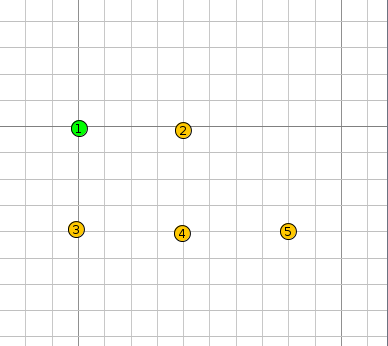
\includegraphics[width=\textwidth]{res/5_nodes}
        \caption{5 nodes}
    \end{subfigure}
    ~
    \begin{subfigure}[b]{0.45\textwidth}
        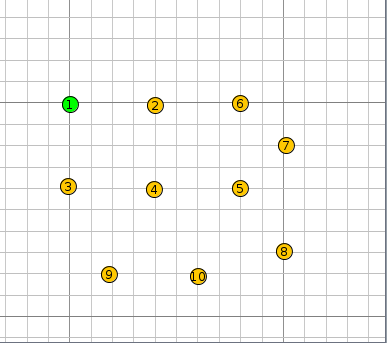
\includegraphics[width=\textwidth]{res/10_nodes}
        \caption{10 nodes}
    \end{subfigure}
    ~
    \begin{subfigure}[b]{0.45\textwidth}
        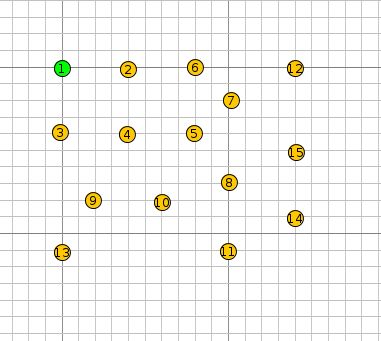
\includegraphics[width=\textwidth]{res/15_nodes}
        \caption{15 nodes}
    \end{subfigure}
    ~
    \begin{subfigure}[b]{0.45\textwidth}
        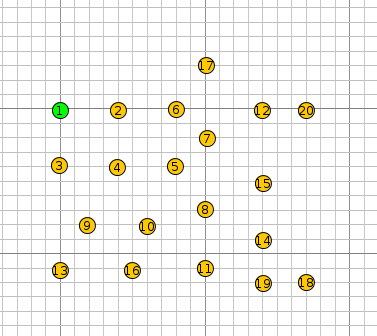
\includegraphics[width=\textwidth]{res/20_nodes}
        \caption{20 nodes}
    \end{subfigure}
    \caption{Position of the nodes}
    \label{fig:nodes_position}
\end{figure}

Also, for each simulation, we keep track of the 4-uple ($t_r$, $t_t$, $t_m$, $t_l$) where $t_r$ is the radio reception time, $t_t$ the radio transmission time, $t_m$ the time the Cpu is working, and $t_l$ the time the Cpu is in low power mode. This 4-uple was recorded for each minute. This gave an idea on how the energy consumption evolved minute by minute.\\

Our tests were done solely on simulation using the Cooja simulation software. The radio model was the default one offered by Cooja which is the \acrfull{udgm}. This radio model abstracts the radio transmission range as circles. The nodes used during the simulations were the \textit{Zolertia Z1} as they proved to have sufficient memory for our code. However, we do want to emphasize that we did not set as a goal to minimize the memory footprint of our code. Optimizations are thus possible to further decrease the code size, and thus maybe reduce the cpu load also. We also considered a setup for all configurations where the radio loss was null. Additionally, all motes were fixed by position, meaning they did not move during the simulation.

\chapter{Results}

After having presented our methodology used when testing our solution, this chapter will present and discuss the results obtained from it.

\section{Energy consumption}

The Fig.\ref{fig:average_energy} shows the average energy consumption in terms of \acrfull{mj} by minute for the nodes. The bar charts show the evolution of the energy consumption with an increasing number of nodes (5, 10, 15 and 20) for the three configurations \textit{simple}, \textit{tipfix} and \textit{aggrega}. As a reminder, the \textit{simple} configuration has no monitoring done with TinyIPFIX while the two has monitoring activated by the mean of TinyIPFIX messages. The difference between \textit{tipfix} and \textit{aggrega} configurations lies in the fact that the \textit{aggrega} has aggregator nodes that merge TinyIPFIX messages into one. \\

\begin{figure}[h]
  \centering
  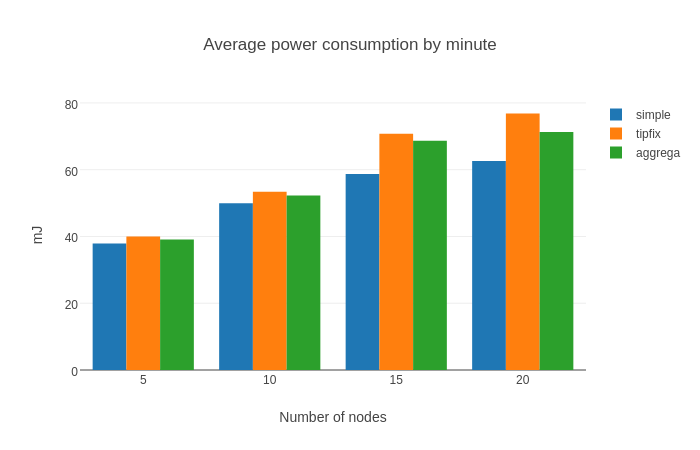
\includegraphics[width=\textwidth]{res/average_energy.png}
  \caption{Average energy consumption in mJ by minute}
  \label{fig:average_energy}
\end{figure}

From the chart, we can conclude that by using aggregators inside the network we can reduce the added energy consumption induced by the usage of TinyIPFIX messages for monitoring purposes. As can be clearly seen when introducing more nodes, the energy consumption increases much more when not using aggregators. The graph on Fig.\ref{fig:increase_energy} shows exactly how the monitoring increase the energy consumption. The increase was computed by comparing the tipfix and aggrega configurations on their counterpart, the simple configuration which does not send any information about the status of the network. As one may notice, the tipfix configuration consumes relatively more energy when the number of nodes increases. However, it appears not to be the case with the aggrega one. Reasons may be due to the positions of the aggregators that impact greatly how the network behaves and thus weight on the power consumption. By placing intelligently the aggregators it is therefore possible to stress the network less.\\

\begin{figure}[h]
  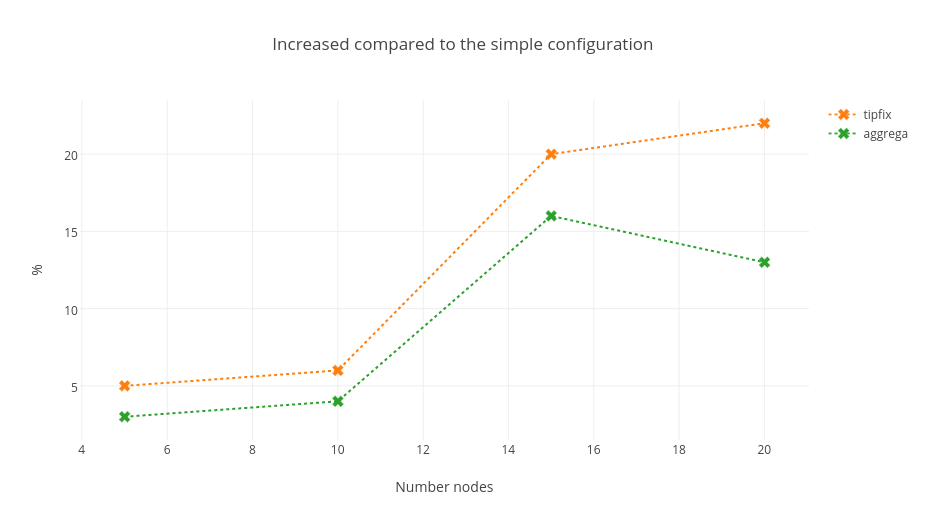
\includegraphics[width=\textwidth]{res/increase_energy.png}
  \caption{Increase in energy consumption induced by monitoring}
  \label{fig:increase_energy}
\end{figure}

One of the big advantages of also using aggregators is that it reduces drastically the load on the nodes that simply export data and does not merge messages. This is depicted in Fig.\ref{fig:aggrega_energy}. The bar chart represents the energy consumption for the exporters and the aggregators in the aggrega configuration. Apart from the case with 5 number of nodes, all the cases show clearly that the exporters consume less energy than the aggregators with almost 20 mJ of difference for 15 nodes.\\

\begin{figure}[h]
  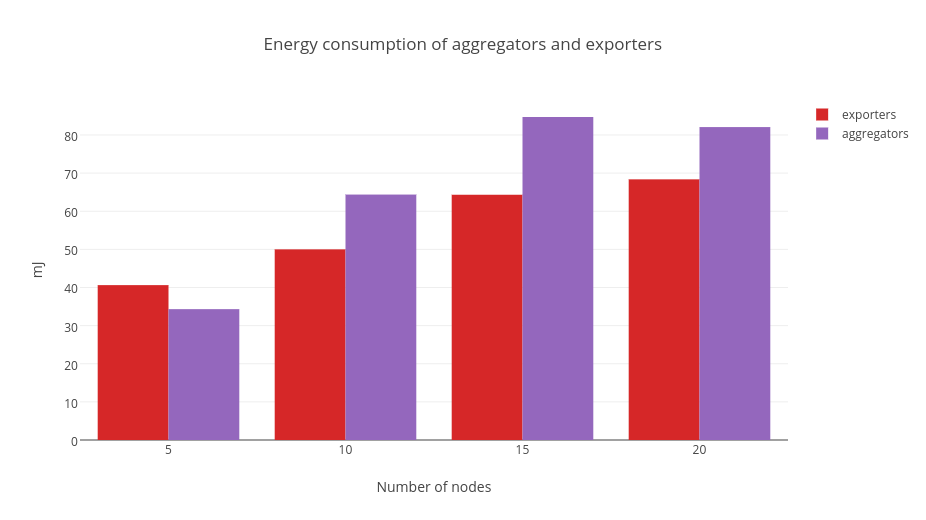
\includegraphics[width=\textwidth]{res/energy_aggrega}
  \caption{Energy consumption between aggregators and exporters}
  \label{fig:aggrega_energy}
\end{figure}

With those results, one may wonder how it affects the battery life of the nodes. The estimated lifetime of the battery is indicated in Tab.\ref{tab:battery_lifetime}. To compute those estimations, we used the following formula :

\begin{equation}
  lifetime = \frac{2400 \acrshort{mah} * 2}{X \acrshort{mw} * 24 hours}
\end{equation}

where $X$ is the power consumption of a node. We used $2400mAh$ as we considered that the nodes were powered by AA battery. We multiply it by $2$ as the \textit{Zolertia Z1} uses 2 batteries. \\

The table clearly shows that to preserve the battery lifetime, aggregators become a must, the more nodes are present in the IoT network.

\begin{table}
  \centering
  \begin{tabular}{|c|c|c|c|c|}
    \hline
    configuration & 5 nodes & 10 nodes & 15 nodes & 20 nodes \\
    \hline
    simple & 317 days & 240 days & 204 days & 190 days\\
    \hline
    tipfix & 300 days & 224 days & 168 days & 156 days\\
    \hline
    aggrega (exporters) & 294 days & 240 days & 186 days & 174 days \\
    \hline
  \end{tabular}
  \caption{Battery lifetime for different configurations}
  \label{tab:battery_lifetime}
\end{table}

\section{Nodes time repartition}

For the purpose of better understanding the power consumption induced by our solution, there is a need to see how often the nodes are active, and when it is the case, what are they doing. To do so, we kept track on the time the nodes spend with their microprocessor active or in low power mode but also the time they were transmitting or receiving data via radio. This is what Fig.\ref{fig:time_all} shows. The Fig.\ref{fig:cpu_time} shows the average time the microprocessor is active by minute while Fig.\ref{fig:lpm_time} shows the average time the microprocessor is in low power mode. Fig.\ref{fig:tx_time} and Fig.\ref{fig:rx_time} shows average transmission time and receiving time by minute for a node. \\

\begin{figure}[h]
    \centering
    \begin{subfigure}[b]{0.45\textwidth}
        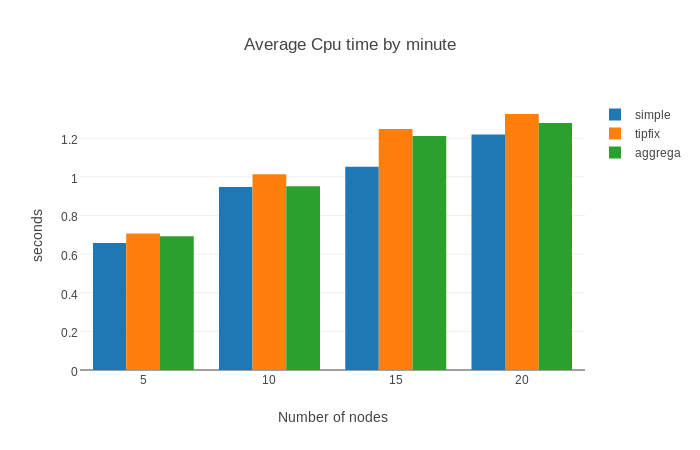
\includegraphics[width=\textwidth]{res/average_cpu}
        \caption{Average time spent with CPU active}
        \label{fig:cpu_time}
    \end{subfigure}
    ~
    \begin{subfigure}[b]{0.45\textwidth}
        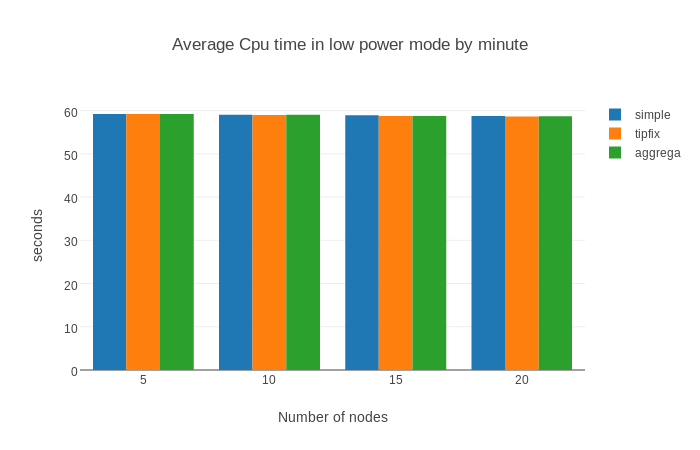
\includegraphics[width=\textwidth]{res/average_lpm}
        \caption{Average time spent with CPU in low power mode}
        \label{fig:lpm_time}
    \end{subfigure}
    ~
    \begin{subfigure}[b]{0.45\textwidth}
        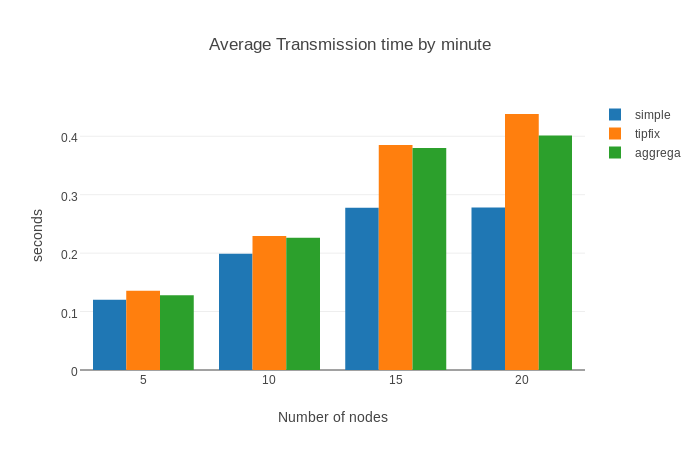
\includegraphics[width=\textwidth]{res/average_tx}
        \caption{Average time spent in transmission mode}
        \label{fig:tx_time}
    \end{subfigure}
    ~
    \begin{subfigure}[b]{0.45\textwidth}
        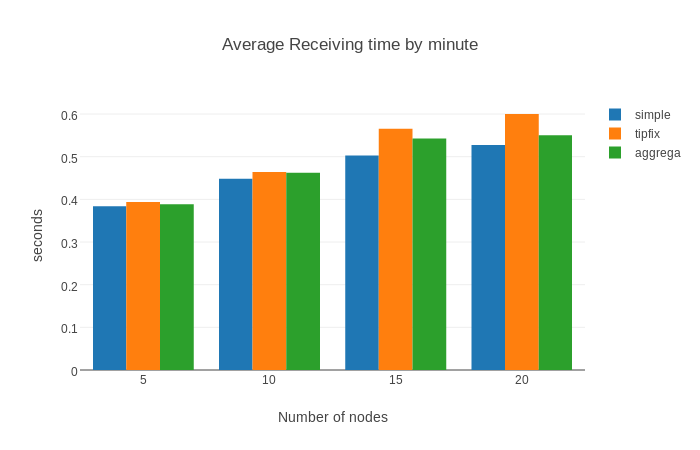
\includegraphics[width=\textwidth]{res/average_rx}
        \caption{Average time spent in receiving mode}
        \label{fig:rx_time}
    \end{subfigure}
    \caption{Average components time of nodes}
    \label{fig:time_all}
\end{figure}

The differences between the three configurations is highly visible for the transmission time and receiving time. In Fig.\ref{fig:tx_time} that shows the transmission time, we can clearly see that, by monitoring, nodes pass more time transmitting data, which influences the receiving time of the nodes. On Fig.\ref{fig:rx_time}, that shows the receiving time, we can see that nodes receive more data that needs to be routed. It is however in the transmission time that there is the largest gap between the configurations with and without TinyIPFIX.\\

However, when analyzing the time spent with the CPU active on Fig.\ref{fig:cpu_time}, we can notice that there is only a marginal difference between configurations with and without TinyIPFIX. This is also seen in Fig.\ref{fig:lpm_time}, that showcases the time the CPU is in low power mode. We can only conclude than the differential of energy consumption lies in the radio usage of the nodes induced by the sending of monitoring data. Increasing the interval at which nodes send their data could be a solution for network imposing as requirement a high battery lifespan.\\

We must emphasize the fact that using aggregators reduced the average time spent by the nodes transmitting or receiving, but also with CPU being active or in low power mode. The fact that TinyIPFIX messages are grouped into one aggregator that merges them into one packet reduces the overhead caused by multiple headers from TinyIPFIX itself but also 6LoWPan.


\chapter{Discussion}

The topics covered by this chapter will be about :

\begin{itemize}
	\item \textbf{Nfsen} We started our master thesis by trying to implement a plugin for that particular software. Details will be given on how this tool works and reasons will be given on why we abandoned the idea of implementing an Nfsen plugin. However, as you will see, our architecture resembles a lot to that of Nfsen.
	\item \textbf{Possible extensions} Those are features that could be added to our current software as to improve it.
	\item \textbf{Security} Issues about security will be addressed.
  \item \textbf{Further works} This will mainly focus on how to improve the data retrieval of meta information about the network.
\end{itemize}

\section{Nfsen, A Graphical Web Tool}

\begin{figure}[!h]
	\centering
	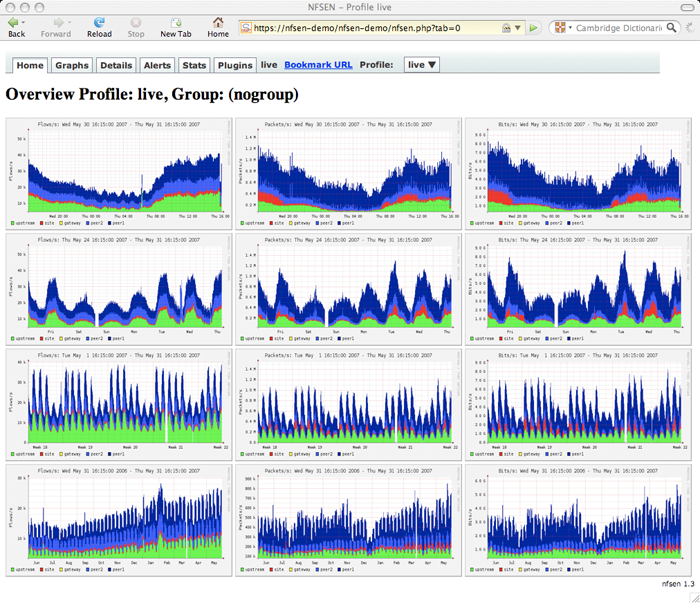
\includegraphics[width=0.8\textwidth]{res/nfsen.png}
	\caption{The Nfsen interface (source : \url{Nfsen.sourceforge.net})}
	\label{fig:Nfsen}
\end{figure}

The subject of our master thesis having been proposed by Professor Sadre last year and being about monitoring flows in IoT networks, the first tool that was presenting itself to us was Nfsen. Per its official website, \textit{Nfsen is a graphical web based front end for the Nfdump Netflow tools}. The Nfsen tool uses various graphs and charts to display the traffic of data varying with a specified time span or time interval. It works with the processing capabilities of Nfdump, a data processing tool using Netflow flows that have been retrieved from a network. Specifically, the Nfsen interface also allows to create plugins to have more ways of displaying data information. At first, it was proposed in the description of the subject of the thesis to use Nfsen along with Nfdump, particularly creating an Nfsen addon to show further information along with what Nfsen already is displaying in terms of graphical content. By plugin, one graphical content that Nfsen is lacking is the current topology of the monitored network, which can be added by making a plugin which extends the graphical tool.\\

In this section, we will explain all the underlying layers of Nfsen, from data exchanged in the monitored network to the graphical web page. We will also discuss our thought process about using Nfsen and the reasons why we have not used it in the end.\\

The first step towards monitoring is data collecting. As we explained in Chapter 3, Netflow is used for collecting flows we are interested in, according to some specific attributes such as the source and destination addresses. Once the flow are captured, they are stored and waiting to be processed. \\

In reality, when the structure of the Netflow data is defined, the flows are actually captured by \textit{nfcapd}, a \textit{Netflow capture deamon}. With nfcapd, the flows are read from the network and the collected data is stored into files, data being split in files according to time slices. Each five minutes, nfcapd outputs a new file where data is stored, named with the current timestamp. One nfcapd process is used for each existing Netflow stream that we want to capture.\\

As seen in the Fig.\ref{fig:Nfdump}, the next important component is \textit{Nfdump}. Nfdump is a command line based tool that provides further data processing. Basically, it reads the data that was previously captured and stored by nfcapd. With Nfdump, data is aggregated and it provides further statistics about the traffic. Nfdump can either analyze the data coming from a single file, or from several of them by concatenating them before analyzing. One strength of Nfdump is that it can filter out the attributes in the data that are not needed during the processing. Afterwards, the data is output either as a text file or binary data, thus being ready for further analysis. Nfdump aggregates and then creates statistics about the flows information stored, such as traffic volume sent during a timelapse. Nfdump thus acts as the backend of Nfsen.\\

\begin{figure}[!h]
	\centering
	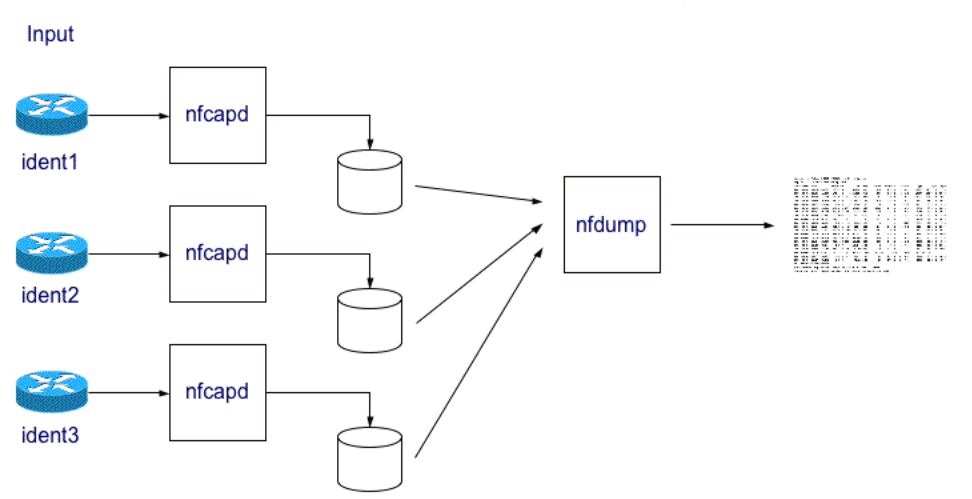
\includegraphics[width=0.8\textwidth]{res/nfdump.png}
	\caption{The Nfdump Structure (source : \url{Nfdump.sourceforge.net})}
	\label{fig:Nfdump}
\end{figure}

Once the data is processed, it is displayed by Nfsen with the help of graphs. Nfsen displays the collected Netflow data, either in flows, packets, or bytes. As you can see in figure \ref{fig:Nfsen}, it can display various types of data, for example data sent through different protocols such as UDP, TCP, etc. It also uses time spans to select which data traffic is to be displayed (being the same time spans where Nfdump did all the processing).\\

As stated earlier, Nfsen can also be extended, by creating plugins. There exist two kinds of plugins. There are the backend plugins that are written in Perl, that are created to add more functions and functionalities such as alerting conditions and data processing. On the other hand, frontend plugins are written in PHP and used to create new display fashions that the original Nfsen application would lack. In our case, we wanted to display the topology of the network under analysis, which Nfsen is not showing in its original state. Note that each backend plugin should be associated with its respective frontend plugin.

\subsection{Nfsen \& Nfdump, not best suited?}

We talked before about Nfsen and how it is possible to create plugins to have further monitoring capabilities. As stated, the first description of the thesis was to create an \textit{Nfsen plugin} to visualize an IoT network in an Ad Hoc manner, with devices having Netflow activated.\\

At the beginning of this school year, once we started working on our thesis, we dug into Nfsen and its functionalities, trying to get familiar with it. First of all, setting up the Nfsen tool showed itself to be very tedious and challenging, as many installation tutorials did not work for all computers and OSs, and had different instructions.\\

The main reason why Nfsen is useful is that it easily and immediately treats the Netflow information retrieved by nfcapd and Nfdump, with little to no addition and/or modification needed. However, as we had decided to design our own IPFIX fields to visualize IoT networks according to our needs, we also had to modify Nfdump. Namely, two fields that the original IPFIX structure does not monitor, and hence are not standardized fields, are the battery level of devices and the parent of each mote in the IoT networks. Digging into Nfdump seems to require quite some time and some knowledge of the Perl language. Entering the last year of our master thesis, we also had never used nor learned the PHP and Perl languages in contrary to Javascript with the Node.js framework. \\

Thinking of using the Node.js framework seemed reasonably more practical in our case in terms of time allocation, since we required to modify the Netflow information retrieved from networks. With further discussion, we decided to write a Javascript program that played the role of Nfdump to efficiently parse and store the Netflow information captured. Similarly, instead of using Nfsen as the graphical interface, we programmed a web server with Node.js to be able to visualize information in which we are interested in. Of course, our graphical interface is less complete than Nfsen's, but it contains a topology showcase that Nfsen does not, that we have programmed using the D3.js library.\\

In the end, Nfsen used with Nfdump present a lot of advantages, as most of the work is already present in its core, only a few things have to be added, i.e. the topology here. It contains a lot of graphical information on how much traffic passes through the network, with many filters such as graphs split according to which protocols send the information. But for the reasons we have cited above, we have decided not to use it and opted for a solution using Node.js.

\section{Possible Extensions}

\subsection*{Monitoring any IPFIX messages}

We will hereby discuss how the server would handle IPFIX messages received from traditional networks or any IPFIX message. As we explained in the description of our solution, the server is able to collect and store logs of the information received from networks. At this step, it is able to parse any IPFIX messages as long as it follows the standard. However the issue arise when wanting to extract informations coming from those IPFIX messages. At the time of writing, the current product considers a flow to be described by the source node id, the destination node id, the number of octets and the number of packets. However traditional networks use IPv4 or IPv6 address as a mean to identify devices in the network. Thus, so as to process correctly those IPFIX messages, we should handle a flow to be described by IPv4 or IPv6 addresses for the source and the destination as well. Another solution would be to not use the node id but instead also the Ipv6 addresses of the nodes. However this solution would imbue a cost as an IPv6 address is stored on 16 bytes. \\

As the purpose of this thesis was IoT network monitoring, our server does not currently process IPFIX messages from traditional networks. Nevertheless, modifying its processing capability to be able to correctly use IPFIX messages with IPv6 addresses as source and destination is not too challenging and is definitely a possible extension. \\

\subsection*{Topology according to real position}

As of now, the topology feature showcases a network topology that only depends on the routing routes, no matter what is the relative position of those motes according to others in the network. \\

A possible extension could be to showcase a topology where its nodes are positioned as in real life, with a corresponding proportional distance. However, that would imply adding complexity on each mote to have a feature computing the coordinates relative to a base point, and that would also induct a raise in traffic volume since more packets containing position information are to be exchanged.

\subsection*{Network failure and Network changes}

When developing the software, we have not made any assumption that links and nodes may potentially fail. As of now, the way the topology updates itself is by refreshing the page and thus showcasing the topology. The topology is built according to IPFIX packets that are sent from the network to the server, which is everytime the server receives a flow of IPFIX packets. In reality, a topology change may come from a link failure, i.e. two nodes may have difficulties communicating together, or node failures if a mote runs out of battery or is accidently broken. \\

One important aspect to take into account is the fact that the topology is organized as a tree, meaning for each node or link failing, there is a cascade of nodes down branches that will consequently not be able to communicate with the gateway node. Of course, the gateway node is a \textit{Single Point of Failure} (see figure \ref{fig:spof}), since it failing would completely cut the communication between the IoT network and the server, thus not having any information on the network anymore.\\

\begin{figure}[!h]
	\centering
	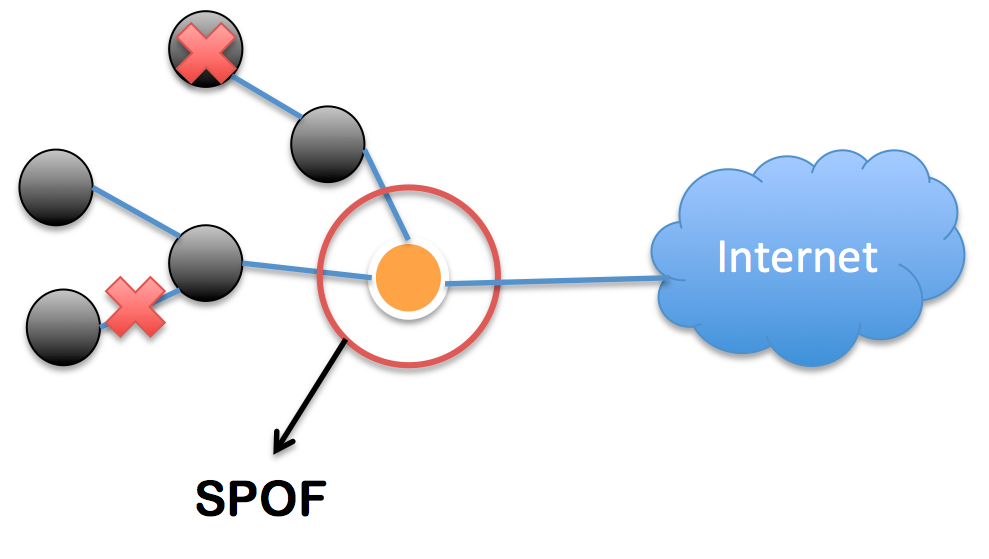
\includegraphics[width=0.8\textwidth]{res/spof.png}
	\caption{Tree topology, link and node failure, SPOF}
	\label{fig:spof}
\end{figure}

A potential extension could be to have a panel showcasing the \textit{previous topology} after an update of topology, allowing to make comparisons between the current and the previous network state, and thus see if there potentially was an important change in the network.\\

As stated, the topology is updated according to Netflow packets and information retrieval. In the network's current state, a mote that has not sent information for a while or a mote that has failed and that has consequently not sent any information would be interpeted the same way in our topology. \\

Further mechanisms are needed to be able to distinguish the two situations, such as adding some field in our TinyIPFIX structure to represent the loss of a neighbors. Plus, it allows to have some information on downstream nodes and send that information to the gateway node. Those solutions require more lines of code on each mote, and a modified IPFIX structure with added fields.

\subsection*{Protocols distribution}

As of now, our software does not have the possibility to sort the flows by protocols (RPL, UDP, TCP, ...). An improvement of our solution could permit to differentiate flows depending on the protocols. However, to effectively enable such feature, the records sent by the nodes should contain more data. Plus, the flow tables stored on nodes would increase due to the fact that flows having the same source and destination could be different based on the protocol used. This implies that the nodes would send more data and a study of the impact on the nodes battery life would be necessary.

\subsection*{Time range}

A possible extension would be to allow an user to select a specific time range to analyze as it is possible with Nfsen. In the traffic volume page, it would show amount of traffic and the statistics for that particular interval of time.

\section{Security}

Throughout the thesis, security has not been the main point of focus. Indeed, we have not implemented any security mechanism, inside the IoT network nor between the gateway node and our server. Data not being encrypted may be an issue as the communication between devices in the network becomes a target for sniffing and packets tempering. Of course, one direct impact of such insecurity is that data to be processed that is sent to the server may be tempered and thus, later on, the monitoring software would showcase wrong information about the traffic load and the topology for example.\\

Purely from a theoretical point of view, there is also a lack of security between devices inside the network, but also between the gateway mote and the server, communicating via UDP. The sniffing of exchanged packets can be an issue, as well as identity theft (spoofing) where a third party could act as, for instance, being the gateway mote and send data to the server, because of the lack of authentication when communication is opened. \\

Authentication mechanisms and encryption are the way to go to solve these problems. We would thus have authentication between motes, and encryption of data when creating packets from motes. However, those mechanisms add lines of codes uploaded on motes, which must be taken into account when analyzing and optimizing performances of the IoT network. In consequence, the mechanisms also add more traffic load to the network.\\

All those points are to be taken into account to showcase accurate data. In our case though, no tempering was possible, as we knew exactly what kind of data passes through the network and which device creates the flows.

\section{Further Works}

Those further works will mainly be focus on improving the meta information extraction from the nodes.\\

The tests shown in the previous chapters were limited to 20 nodes at maximum due to the constraint imposed from the computer used during simulation. However, 20 nodes is quite a small network. Our tests should be improved and tested on bigger networks ranging from hundreds to thousands of nodes. Additionally, the solution should be tested on real nodes and real network so as to confront our solution with real environments and applications. By increasing the number of tests, some parameters should also be highlighted. One of those parameters that should come out should be, we think, the average depth of the network. By depth we means the number of nodes that should reroute a message coming from a leaf node (without children) to the gateway node.\\

Also our tests supposed that there was no packet loss. This could be applicable to reliable network to a limit of 90\% packet loss ratio but WSN are not to be considered reliable. They are lossy by nature. Thus it would be great to study the impact made by resending messages in case of dropped packets. We could envision for that using a solution like \acrshort{mqtt} \cite{website:mqtt} or simply send messages via TCP and not UDP.\\

A standard should also be worked upon to as to use a common message format from data coming from nodes. IPFIX or TinyIPFIX could be that standard. In this master thesis we used TinyIPFIX to monitor the network. But it was developed at first to send sensors values (humidity, temperature, ...). TinyIPFIX appears to be a versatile solution that could permit monitoring of IoT networks in term of traffic information but also in term of sensors values. The standardization should be done by defining common fields.\\

Optimizations could also be done in the triggering of the message. As of now, we use a fixed interval time set beforehand. But what if the nodes could communicate between themselves and set by themselves the best interval time so as to optimize battery lifetime. Plus, so as to not provoke congestion, nodes could send data at different time. This is a concern that will mostly arise with large networks.\\

In conclusion many improvements can be made as to enhance our solution. Those solutions should have as goal to reduce the energy consumption while not decreasing the informations extracted.
